%Master File:lectures.tex

\lesson{Integral Calculus}
\vspace{-1cm}
\begin{center}
  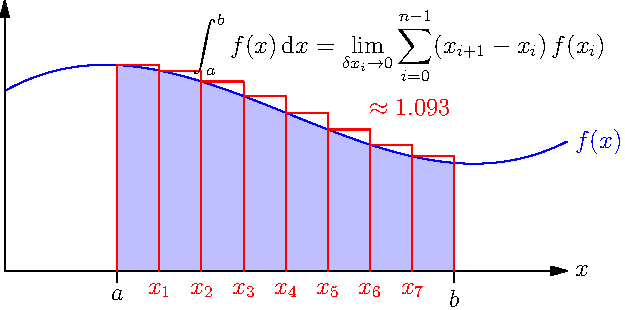
\includegraphics[height=10cm]{riemann-2}
\end{center}
\keywords{Riemann Integration, integration by parts, gaussian integrals}
%%%%%%%%%%%%%%%%%%%%%%% Next Slide %%%%%%%%%%%%%%%%%%%%%%%
\renewcommand{\Outline}{%
\begin{slide}
\section[1]{Outline}

\begin{minipage}{10cm}\raggedright
  \begin{enumerate}\squeeze
    \outlineitem{Defining Integrals}{integration}
    \outlineitem{Doing Integrals}{integration}
    \outlineitem{Gaussian Integrals}{gaussian}
  \end{enumerate}
\end{minipage}\hfill
\begin{minipage}{12cm}
  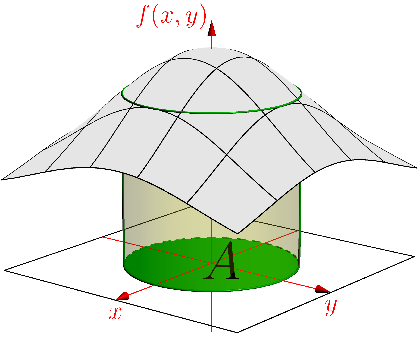
\includegraphics[width=12cm]{multidimint}
\end{minipage}
\end{slide}
\addtocounter{outlineitem}{1}
}

\setcounter{outlineitem}{1}


%%%%%%%%%%%%%%%%%%%%%%% Next Slide %%%%%%%%%%%%%%%%%%%%%%%
\Outline % Introduction
%%%%%%%%%%%%%%%%%%%%%%% Next Slide %%%%%%%%%%%%%%%%%%%%%%%

\begin{slide}
\section{Riemann Integral}

\pb
\begin{itemize}
\item Integrals represent area beneath a curve\pauseh
\end{itemize}

\begin{center}
  \multipdf[width=0.9\linewidth]{riemann}\pause
\end{center}

\end{slide}

%%%%%%%%%%%%%%%%%%%%%%% Next Slide %%%%%%%%%%%%%%%%%%%%%%%

\begin{slide}
\section[-2]{Linearity of Integration}

\begin{PauseHighLight}
  \begin{itemize}
  \item Integration is a linear operator
    {\small
    \begin{align*}
      \int_a^b \bra{r\,f(x) + s\,g(x)} \, \dd x
      &= \lim\limits_{\delta x_i\rightarrow 0} \sum_{i=0}^{n-1}
                                    (x_{i+1} - x_i) \, \bra{r\,f(x_i)
        + s\,g(x_i)} \pause \\
      &= \lim\limits_{\delta x_i\rightarrow 0} \bra{
        \sum_{i=0}^{n-1} (x_{i+1} - x_i) \, r\,f(x_i)
        + \sum_{i=0}^{n-1} (x_{i+1} - x_i) \, s\,g(x_i)} \pauseb \\
      &= \lim\limits_{\delta x_i\rightarrow 0} \bra{
        r\,\sum_{i=0}^{n-1} (x_{i+1} - x_i) \, f(x_i)
        + s\, \sum_{i=0}^{n-1} (x_{i+1} - x_i) \, g(x_i)} \pauseb \\
        &=  r\, \lim\limits_{\delta x_i\rightarrow 0} \sum_{i=0}^{n-1}
          (x_{i+1} - x_i) \, f(x_i)
          +  s\, \lim\limits_{\delta x_i\rightarrow 0} \sum_{i=0}^{n-1}
          (x_{i+1} - x_i) \, g(x_i) \pauseb \\
      &= r \int_a^b f(x) \, \mathrm{d}x + s \int_a^b f(x) \, \mathrm{d}x\pauseb
    \end{align*}}
  \end{itemize}
\end{PauseHighLight}

\end{slide}

%%%%%%%%%%%%%%%%%%%%%%% Next Slide %%%%%%%%%%%%%%%%%%%%%%%

\begin{slide}
\section[-2]{Fundamental Law of Calculus}

\begin{PauseHighLight}
  \begin{itemize}
  \item Let
    \begin{align*}
      I(a,x) =  \int_a^x f(z) \, \mathrm{d}z =  \lim\limits_{\delta z_i\rightarrow 0} \sum_{i=0}^{n-1}
          (z_{i+1} - z_i) \, f(z_i)\pause
    \end{align*}
  \item Now for small $\delta x$
    \begin{align*}
      I(a,x+\delta x) =  \int_a^{x+\delta x} f(z) \, \mathrm{d}z
      =  \lim\limits_{\delta z_i\rightarrow 0} \sum_{i=0}^{n-1}
      (z_{i+1} - z_i) \, f(z_i) + \delta x \, f(x)
    \end{align*}
  \item Thus
    \begin{align*}
      \frac{\dd I(a, x)}{\dd x}
      &= \lim_{\delta x\rightarrow 0} \frac{I(x+\delta x) - I(x)}{\delta x} \pause 
      = \lim_{\delta x\rightarrow 0}\frac{\delta x \, f(x)}{\delta x} \pauseb = f(x)\pauseb
    \end{align*}
   \end{itemize}
\end{PauseHighLight}


\end{slide}

%%%%%%%%%%%%%%%%%%%%%%% Next Slide %%%%%%%%%%%%%%%%%%%%%%%

\begin{slide}
 \section[-2]{The Other Way Around}

  \begin{PauseHighLight}
  \begin{itemize}
  \item Consider
    {\small
    \begin{align*}
      \int_a^b \frac{\dd f(x)}{\dd x} \dd x
      &= \int_a^b  \lim_{\delta x\rightarrow 0} \frac{f(x+\delta x) -
        f(x)}{\delta x} \dd x \pause\\
      &= \lim_{x_{i+1}-x_i\rightarrow 0}  \sum_{i=0}^{n-1} \bra{x_{i+1}- x_i} \frac{f(x_{i+1})
        - f(x_i)}{x_{i+1}- x_i}\pauseb\\
      &=  \lim_{x_{i+1}-x_i\rightarrow 0}  \sum_{i=0}^{n-1} \bra{f(x_{i+1})
        - f(x_i)}\pauseb\\
      &= \bra{f(x_1)- f(x_0)} + \bra{f(x_2)- f(x_1)} + \bra{f(x_3)-
        f(x_2)} + \cdots \\
      & \quad + \bra{f(x_{n-1})- f(x_{n-2})} + \bra{f(x_n)-
        f(x_{n-1})} \pauseb \\
      &= f(x_n) - f(x_0)\pauseb = f(b) -f(a)\pauseb
    \end{align*}}
  \item We can think of integration as an \emph{anti-derivative} it
    undoes differentiation\pauseb
  \end{itemize}
\end{PauseHighLight}

\end{slide}

%%%%%%%%%%%%%%%%%%%%%%% Next Slide %%%%%%%%%%%%%%%%%%%%%%%

\begin{slide}
\section[-1]{Indefinite Integrals}
  
\begin{PauseHighLight}
  \begin{itemize}
  \item So far we have considered \emph{definite integrals} where we
    integrate between two points ($a$ and $b$)\pause
  \item However, when think about integration as an
    anti-derivative, it is useful to think of a function
    $F(x)= \int f(x) \, \dd x$\pause
  \item So that $F'(x) = f(x)$\pause
  \item However the function $F(x)$, $F(x)+1$, $F(x)+\pi$, etc.{} all
    have the same derivative so $F(x)$ is only defined up to an
    additive constant\pause
  \item Note that the definite integral is given by
    \begin{align*}
      \int_a^b f(x) \dd x = F(b) - F(a)\pause
    \end{align*}
  \end{itemize}
\end{PauseHighLight}

\end{slide}


%%%%%%%%%%%%%%%%%%%%%%% Next Slide %%%%%%%%%%%%%%%%%%%%%%%

\begin{slide}
\section[-2]{Multiple Integrals}

\begin{PauseHighLight}
  \begin{itemize}
  \item For functions involving many independent variables
    (e.g. $f(x,y)$, $f(x,y,z)$, $f(\bm{x})$) we can integrate over
    multiple dimensions\pause
  \item For example
    \vspace*{-3cm}

    \begin{align*}
      \iint\limits_A f(x, y)\, \dd x\, \dd y \hspace{3cm}\raisebox{-3cm}{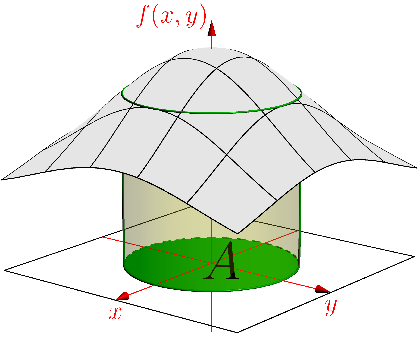
\includegraphics[height=8cm]{multidimint}}\pause
    \end{align*}
  \item It gets tedious writing multiple integral signs and I tend to
    write just one
    \begin{align*}
     \int\cdots\int f(x_1, x_2,\ldots, x_n)  \, \dd x_1\, \dd
      x_2\cdots \dd x_n\pause
      =  \int f(\bm{x}) \, \dd \bm{x} \pauseb
    \end{align*}
  \end{itemize}
\end{PauseHighLight}


\end{slide}

%%%%%%%%%%%%%%%%%%%%%%% Next Slide %%%%%%%%%%%%%%%%%%%%%%%
\Outline % Doing Integrals
%%%%%%%%%%%%%%%%%%%%%%% Next Slide %%%%%%%%%%%%%%%%%%%%%%%

\begin{slide}
\section{Performing Integration}

\begin{PauseHighLight}
  \begin{itemize}
  \item A key method for performing integrals is through knowledge of
    the anti-derivative\pause
  \item If we know $F'(x) = f(x)$ then $F(x) + c = \int f(x)\, \dd
    x$\pause
  \item E.g. we know that $\dd x^n/ \dd x = n\, x^{n-1}$ therefore
    \begin{align*}
      \int x^{n-1} \, \dd x = \frac{1}{n} \int \frac{\dd x^{n}}{\dd x}
      \dd x \pause= \frac{x^n}{n}\pauseb + c\pauseb
    \end{align*}
    and
    \begin{align*}
      \int_a^b x^{n-1} \, \dd x = \frac{b^n}{n} - \frac{a^n}{n} \pause
    \end{align*}
  \end{itemize}
\end{PauseHighLight}

\end{slide}

%%%%%%%%%%%%%%%%%%%%%%% Next Slide %%%%%%%%%%%%%%%%%%%%%%%

\begin{slide}
\section[-2]{Is Integration Straightforward?}

\begin{PauseHighLight}\squeeze
  \begin{itemize}
  \item We saw due to the product and chain rules that we can
    differentiate almost anything\pause.  Given integration is the
    anti-derivative can we integrate anything?\pauseb
  \item Products and compositions
    \begin{align*}
      \int f(x) \, g(x) \, \dd x &=\; ? &  \int f(g(x)) \, \dd x  &= \;?\pause
    \end{align*}
  \item Unfortunately, unlike differentiation we don't have a small
    parameter we can expand in\pause
  \item In general integration is hard\pause
  \end{itemize}
\end{PauseHighLight}

\end{slide}

%%%%%%%%%%%%%%%%%%%%%%% Next Slide %%%%%%%%%%%%%%%%%%%%%%%

\begin{slide}
\section{Integration by Parts}

\begin{PauseHighLight}
  \begin{itemize}
  \item Recall the product rule $\frac{\dd f(x)\, g(x)}{\dd x} =
    \frac{\dd f(x)}{\dd x}\,{\scriptstyle g(x) + f(x)}\, \frac{\dd g(x)}{\dd x}$\pause
  \item Integrating we get
    \begin{align*}
      \int_a^b \frac{\dd f(x)\, g(x)}{\dd x} \, \dd x
      &= \int_a^b  \frac{\dd f(x)}{\dd x}\, g(x) \, \dd x 
        + \int_a^b  f(x)\, \frac{\dd g(x)}{\dd x}\, \dd x \pause\\
        &= \left[ f(x)\, g(x)\right]_a^b \pauseb = f(b)\,g(b) - f(a)\,g(a)\pauseb
    \end{align*}
  \item Unfortunately we get two integrals\pause, but we can turn this around
    \begin{align*}
      \int_a^b  f(x)\, \frac{\dd g(x)}{\dd x}\, \dd x  = \left[ f(x)\,
      g(x)\right]_a^b  - \int_a^b  \frac{\dd f(x)}{\dd x}\, g(x) \, \dd x \pauseb
    \end{align*}
    whether this is helpful depends on $f(x)$ and $g(x)$\pauseb
  \end{itemize}
\end{PauseHighLight}

\end{slide}

%%%%%%%%%%%%%%%%%%%%%%% Next Slide %%%%%%%%%%%%%%%%%%%%%%%

\begin{slide}
\section[-2]{Example of Integration by Parts}

\begin{PauseHighLight}
  \begin{itemize}
  \item Consider
    \begin{align*}
      \Pi(z) &= \int_0^\infty x^z \, \e{-x} \, \dd x\pause = 
      \int_0^\infty x^z \frac{\dd (-\e{-x})}{\dd x} \, \dd x \pauseb\\
      &= \left[ x^z\, (-\e{-x})  \right]_0^\infty - \int_0^\infty 
        \frac{\dd x^z}{\dd x}\, (-\e{-x}) \, \dd x\pauseb\\
             &= \int_0^\infty  (z x^{z-1}) \, \e{-x} \, \dd x \pauseb
               = z\,\int_0^\infty x^{z-1} \,  \e{-x} \,  \dd x \pauseb
               = z\,\Pi(z-1) \pauseb
    \end{align*}
  \item Thus $\Pi(z) = z\, \Pi(z-1)$, but
    \begin{align*}
      \Pi(0) = \int_0^\infty \e{-z} \,\dd z = \left[ -\e{-x}
      \right]_0^\infty\pauseb
      = -\e{-\infty} - (-\e{0}) \pauseb = 1\pauseb
    \end{align*}
  \item Now $\Pi(n) = n\,\Pi(n-1) = n\,(n-1)\,\Pi(n-2) =
    n\,(n-1)\,(n-2)\ldots1 = n!$\pauseb
  \end{itemize}
\end{PauseHighLight}

\end{slide}

%%%%%%%%%%%%%%%%%%%%%%% Next Slide %%%%%%%%%%%%%%%%%%%%%%%

\begin{slide}
\section[-2]{Substitution}
  
\begin{PauseHighLight}
  \begin{itemize}
  \item We can make a transformation from $x$ to $u\pause=u(x)\pauseb$
    \begin{align*}
      \int_a^b f(x) \, \dd x &= \lim_{\delta x_i \rightarrow 0}
      \sum_{i=0}^{n-1} f(x_i) (x_{i+1}-x_i) \pause\\
      &= \lim_{\delta u_i \rightarrow 0}
      \sum_{i=0}^{n-1} f(x(u_i)) \frac{x(u_{i+1})-x(u_i)}
      {u_{i+1}- u_i}   (u_{i+1}- u_i)\pauseb\\
      &= \int_{u(a)}^{u(b)} f(x(u)) \, \frac{\dd x(u)}{\dd u} \, \dd u\pauseb
    \end{align*}
    \begin{itemize}
    \item  where $u_i$ is such that $x(u_i) = x_i$ or $u_i=u(x_i)$
      where $u(x)$ is the inverse of $x(u)$\pauselevel{=4,
        build, highlight}\pause
    \item using $\lim\limits_{\delta u_i \rightarrow 0} \frac{x(u_{i+1})-x(u_i)}
      {u_{i+1}- u_i} = \frac{\dd x(u_i)}{\dd u}$\pauseb
    \end{itemize}
  \end{itemize}
\end{PauseHighLight}

\end{slide}


%%%%%%%%%%%%%%%%%%%%%%% Next Slide %%%%%%%%%%%%%%%%%%%%%%%

\begin{slide}
\section[-2]{Example of Integration by Substitution}

\begin{PauseHighLight}
  \begin{itemize}
  \item We consider $I(n) = \int\limits_0^\infty x^n\, \e{-x^2/2} \, \dd x$\pause
  \item Let $u(x) =x^2/2$ or $x(u) = \sqrt{2\,u}$ so that
    \begin{align*}
      \frac{\dd x(u)}{\dd u} &= \frac{1}{\sqrt{2\,u}} & u(0)&=0 & u(\infty)
                                                            = \infty\pause
    \end{align*}
  \item Thus
    \begin{align*}
      I(n) &= \int_0^\infty \bra{\sqrt{2\,u}}^{n}\e{-u}\, \frac{1}{\sqrt{2\,u}} \, 
      \dd u\pause\\
      &= 2^{\frac{n-1}{2}} \int_0^\infty  u^{\frac{n-1}{2}} \, \e{-u}\,
      \dd u \pauseb = 2^{\frac{n-1}{2}}\,\, \Pi\!\bra{\frac{n-1}{2}}\pauseb
    \end{align*}
  \item $I(1) = 1$\pauseb, $I(3)=2\times1!=2$\pauseb,
    $I(5)=2^2\times2!=8$\pauseb, but $I(0)=
    \Pi(-1/2)/\sqrt{2}$\pauseb, $I(2)= \sqrt{2}\,\Pi(1/2)=
    \Pi(-1/2)/\sqrt{2}$\pauseb
  \end{itemize}
\end{PauseHighLight}

\end{slide}


%%%%%%%%%%%%%%%%%%%%%%% Next Slide %%%%%%%%%%%%%%%%%%%%%%%

\begin{slide}
  \section[-2]{Changing Variables in Multidimensional Space}

\begin{PauseHighLight}
  \begin{itemize}
  \item When changing variables in many dimensions $\bm{x} \rightarrow
    \bm{u}$ the change of variables involves the Jacobian
    {\small
    \begin{align*}
      \int f(\bm{x}) \dd \bm{x}
      &= \int f(\bm{x}(\bm{u})) \, |\det(\mat{J})| \dd \bm{u},
        & \bm{J} &=
          \begin{pmatrix}
            \pd{x_1}{u_1} & \pd{x_1}{u_2} & \cdots & \pd{x_1}{u_n} \\
            \pd{x_1}{u_2} & \pd{x_2}{u_2} & \cdots & \pd{x_2}{u_n} \\
            \vdots & \vdots & \ddots & \vdots  \\
            \pd{x_n}{u_1} & \pd{x_n}{u_2} & \cdots & \pd{x_n}{u_n}
          \end{pmatrix}\pause
    \end{align*}}
  \item E.g. transforming from Cartesian coordinates $(x,y)$ to polar
    coordinates $(r,\theta)$ then $x=r\,\cos(\theta)$ and
    $y=r\,\sin(\theta)$
    {\small
    \begin{align*}
      |\det(\mat{J})| &= \left| \det\!\begin{pmatrix}
            \pd{r\,\cos(\theta)}{r} &  \pd{r\,\cos(\theta)}{\theta}  \\
            \pd{r\,\sin(\theta)}{r} &  \pd{r\,\sin(\theta)}{\theta}  \\
          \end{pmatrix} \right| \pause
    = \left| \det\!\begin{pmatrix}
            \cos(\theta) &  -r\,\sin(\theta)  \\
            \sin(\theta) &  r\,\cos(\theta)  \\
                   \end{pmatrix} \right| \pauseb\\
      &= r\,\bra{\cos^2(\theta) + \sin^2(\theta)}\pauseb = r \pauseb
    \end{align*}}
\item  That is, $\dd x\, \dd y = r\,\dd r\, \dd \theta$\pauseb
  \end{itemize}
\end{PauseHighLight}

\end{slide}
%%%%%%%%%%%%%%%%%%%%%%% Next Slide %%%%%%%%%%%%%%%%%%%%%%%

\begin{slide}
  \section[-2]{Change of Variables in Pictures}

  \pause \pb\pauselevel{=1}
  \begin{center}
    \multipdf[width=0.8\textwidth]{polarCoord}\pause
  \end{center}
\end{slide}

%%%%%%%%%%%%%%%%%%%%%%% Next Slide %%%%%%%%%%%%%%%%%%%%%%%

\begin{slide}
\section[-1]{Differentiating Through the Integral}

\begin{PauseHighLight}
  \begin{itemize}
  \item A trick that sometimes works is differentiating through an
    integral, e.g.{} consider finding moments
    \begin{align*}
      M_n = \av{X^n} = \int_{-\infty}^\infty x^n \, f_X(x) \, \dd x\pause
    \end{align*}
  \item We can define a momentum generating function
    \begin{align*}
      Z(\ell) =  \int_{-\infty}^\infty \e{\ell \, x} \, f_X(x) \, \dd x\pause
    \end{align*}
  \item Then $M_n = Z^{(n)}(0)$
    \begin{align*}
      \left. \frac{\dd^n Z(\ell)}{\dd \ell^n} \right|_{\ell = 0} = 
      \int_{-\infty}^\infty \left. \frac{\dd^n \e{\ell \, x}}{\dd
      \ell^n}  \right|_{\ell = 0}  \hspace{-1em} \, f_X(x) \, \dd x\pauseb
      =  \int_{-\infty}^\infty x^n \, f_X(x) \, \dd x\pauseb = M_n\pauseb
    \end{align*}
  \end{itemize}
\end{PauseHighLight}

\end{slide}

%%%%%%%%%%%%%%%%%%%%%%% Next Slide %%%%%%%%%%%%%%%%%%%%%%%

\begin{slide}
\section{Cumulant Generating Function}
  
\begin{PauseHighLight}
  \begin{itemize}
  \item Note that $\e{\ell\,x} = 1 + \ell\,x + \tfrac{1}{2}
    \ell^2\,x^2 + \tfrac{1}{3!} \ell^3\,x^3 + \cdots$\pause
  \item So
    \begin{align*}
      Z(\ell) =  \int_{-\infty}^\infty \e{\ell \, x} \, f_X(x) \, \dd
      x\pause
      = 1 + \ell\, M_1 + \frac{1}{2} \ell^2\, M_2 +  \frac{1}{3!}
      \ell^3 M_3 + \cdots\pauseb
    \end{align*}
  \item Now using $\log(1+\epsilon) = \epsilon - \tfrac{1}{2}
    \epsilon^2 + \tfrac{1}{3} \epsilon^3 + \cdots$
    {\small
    \begin{align*}
      G(\ell) = \logg{Z(\ell)} = \ell\,M_1 +  \frac{1}{2}
      \ell^2\bra{M_2 - M_1^2} +  \frac{1}{3!}
      \ell^3 \bra{M_3 - 3\, M_2\,M_1 + 2\,M_1^3} + \cdots\pause
    \end{align*}}
  \item So that $\kappa_n=G^{(n)}(0)$, with $\kappa_1=M_1$ (the mean),
    $\kappa_2 = M_2-M_1^2$ (the variance), $\kappa_3 = M_3 - 3\,
    M_2\,M_1 + 2\,M_1^3$ (the third cumulant related to the skewness)\pause
  \end{itemize}
\end{PauseHighLight}

\end{slide}

%%%%%%%%%%%%%%%%%%%%%%% Next Slide %%%%%%%%%%%%%%%%%%%%%%%

\begin{slide}
\section[-1]{More Integration}

\begin{PauseHighLight}
  \begin{itemize}
  \item Although we have a few tricks, integration is hard\pause
  \item Surprisingly integration sometimes is easier when carried out
    in the complex plane\pause
  \item This is a beautiful part of mathematics\pause{} (due largely
    to Cauchy)\pauseb---but beyond the scope of this course\pauseb
  \item Interestingly, also there is an algorithm that allows us to
    integrate a lot of function\pause. It is sufficiently complicated
    that you need to write a computer algorithm of considerable
    complexity to implement it\pauseb.  Most symbolic manipulation
    packages (e.g. Mathematica) have implemented some part of this
    algorithm\pauseb
  \end{itemize}
\end{PauseHighLight}

\end{slide}

%%%%%%%%%%%%%%%%%%%%%%% Next Slide %%%%%%%%%%%%%%%%%%%%%%%

\begin{slide}
\section[-2]{Special Functions}

\begin{PauseHighLight}
  \begin{itemize}
  \item There are integrals with no known closed form solution\pause
  \item We saw that $\Pi(z) = \int\limits_0^\infty x^z\, \e{-x} \, \dd x$
    satisfies $\Pi(z) = z\,\Pi(z-1)$\pause
  \item For integer $n$ then $\Pi(n) = n!$\pause, but for general $z$,
    the integal $\Pi(z)$ can't be written in terms of elementary
    functions\pause
  \item We consider $\Pi(z)$ as a special function in its own
    right\pause
  \item Although, history has left us with the gamma function instead
    \begin{align*}
      \Gamma(z) = \int_0^\infty x^{z-1}\, \e{-x} \, \dd x\pauseb = \Pi(z-1)\pauseb
    \end{align*}
  \item Other special function defined by integrals exist (e.g. the
    Bessel , Aire, hypergeometric, elliptic, error functions, \ldots)\pauseb
  \end{itemize}
\end{PauseHighLight}

\end{slide}


%%%%%%%%%%%%%%%%%%%%%%% Next Slide %%%%%%%%%%%%%%%%%%%%%%%
\Outline % Gaussian Integrals
%%%%%%%%%%%%%%%%%%%%%%% Next Slide %%%%%%%%%%%%%%%%%%%%%%%

\begin{slide}
\section{Gaussian Integrals}

\begin{PauseHighLight}
  \begin{itemize}
  \item Gaussian integrals  are integrals involving $\e{-x^2}$, e.g.
    \begin{align*}
      \int_{-\infty}^\infty \e{-x^2} \, \dd x
      &&
         \int_{-\infty}^\infty x^4 \e{-a\,x^2 - b x}\, \dd x\pause
    \end{align*}
  \item They are important in computing integrals with respect to the
    normal distribution
    \begin{align*}
      \mathcal{N}(x|\mu, \sigma) = \frac{1}{\sqrt{2\, \pi} \, \sigma} \,\e{-(x-\mu)^2/(2\,\sigma^2)}\pause
    \end{align*}
  \item The great news is that these integrals are all doable\pauseb
  \item The bad news is that they are quite tricky to do\pauseb
  \end{itemize}
\end{PauseHighLight}

\end{slide}

%%%%%%%%%%%%%%%%%%%%%%% Next Slide %%%%%%%%%%%%%%%%%%%%%%%

\begin{slide}
\section[-2]{The Gaussian Integral}

\begin{PauseHighLight}\small\squeeze
  \begin{itemize}
  \item The integral over a Gaussian is surprisingly difficult
    \begin{align*}
        I_1 = \int_{-\infty}^{\infty} \e{-x^2/2} \, \dd x\pause
    \end{align*}
  \item There is a nice trick which is to consider
    \begin{align*}
        I_1^2 &=  \int_{-\infty}^{\infty} \e{-x^2/2} \, \dd x
                \int_{-\infty}^{\infty} \e{-y^2/2} \, \dd y
                =   \int_{-\infty}^{\infty}  \int_{-\infty}^{\infty}
                  \e{-(x^2+y^2)/2} \, \dd x \, \dd y\pause
      \end{align*}
    \item Making the change of variables $r
      = \sqrt{x^2 + y^2}$ and $\theta = \arctan(y/x)$  (so that
      $x=r\,\cos(\theta)$, $y=r\,\sin(\theta)$ and $x^2+y^2=r^2$)
      \begin{align*}
        I_1^2 = \int_0^{2\,\pi} \dd \theta \int_{0}^\infty r\,e^{-r^2/2} \, \dd r
        = 2\,\pi \ \int_{0}^\infty r\,e^{-r^2/2} \, \dd r \pause
      \end{align*}
  \end{itemize}
\end{PauseHighLight}

\end{slide}


%%%%%%%%%%%%%%%%%%%%%%% Next Slide %%%%%%%%%%%%%%%%%%%%%%%

\begin{slide}
\section[-1]{The Gaussian Integral Continued}

\begin{PauseHighLight}\small\squeeze
  \begin{itemize}
    \item From before
      \begin{align*}
        I_1^2   = 2\,\pi \ \int_{0}^\infty r\,e^{-r^2/2} \, \dd r
      \end{align*}
    \item Finally let $u=r^2/2$ so that $\dd u/\dd r =
      r$ or $\dd u= r\,\dd r$ we get 
      \begin{align*}
        I_1^2 = 2\,\pi\ \int_{0}^\infty e^{-u} \, \dd u = 2\,\pi\pause
      \end{align*}
    \item So that $I_1 = \sqrt{2\,\pi}$\pauseb
    \item Incidentally, $I_1 = \sqrt{2}\, \Pi(-1/2)$ so $\Pi(-1/2) =
    \Gamma(1/2) = \sqrt{\pi}$\pauseb
  \end{itemize}
\end{PauseHighLight}

\end{slide}


%%%%%%%%%%%%%%%%%%%%%%% Next Slide %%%%%%%%%%%%%%%%%%%%%%%

\begin{slide}
\section[-2]{Normal Distribution}

\begin{PauseHighLight}
  \begin{itemize}
  \item We consider
    \begin{align*}
      I_2 = \int_{-\infty}^{\infty} \e{-(x-\mu)^2/(2\sigma^2)} \dd x\pause
    \end{align*}
  \item Making the change of variables $z=(x-\mu)/\sigma$ so that $\dd z = \dd
      x/\sigma$ or $\dd x = \sigma \dd z$.  Then
      \begin{align*}
        I_2 = \sigma \int_{-\infty}^{\infty} \e{-z^2/2} \dd z =
        \sigma\,I_1 = \sqrt{2\,\pi}\,\sigma\pause
      \end{align*}
    \item Note that the \textit{probability density function} (PDF) for a
      normally distributed random variable is given by
      \begin{align*}
        \mathcal{N}(x\mid \mu, \sigma^2) = \frac{1}{\sqrt{2\,\pi}\,\sigma} \e{-(x-\mu)^2/(2\sigma^2)} \pause
      \end{align*}
  \end{itemize}
\end{PauseHighLight}

\end{slide}


%%%%%%%%%%%%%%%%%%%%%%% Next Slide %%%%%%%%%%%%%%%%%%%%%%%

\begin{slide}
\section[-2]{Multi-dimensional Gaussians}

\begin{PauseHighLight}
  \begin{itemize}
  \item Consider
    \begin{align*}
      I_3 = \int_{-\infty}^\infty \cdots \int_{-\infty}^\infty
      \e{-\frac{1}{2}\|\bm{x}\|_2^2} \dd x_1 \cdots \dd x_n
    \end{align*}
    where $\bm{x} = (x_1, x_2, \ldots, x_n)^\tr$\pause
  \item Note that $\len{\bm{x}}_2^2 = x_1^2+x_2^2+\cdots+x_n^2$ and
    using $\e{\sum_i a_i} = \prod\limits_i \e{a_i}$
  \begin{align*}
    I_3 &= \int_{-\infty}^\infty \cdots \int_{-\infty}^\infty
          \e{-\frac{1}{2}  \sum\limits_{i=1}^n x_i^2} \dd x_1 \cdots \dd
          x_n \pause\\
        &= \prod_{i=1}^n \int_{-\infty}^\infty  \e{-x_i^2/2} \,
          \dd x_i \pauseb =  \prod_{i=1}^n \sqrt{2\,\pi} = (2\,\pi)^{n/2} \pauseb
  \end{align*}
  \end{itemize}
\end{PauseHighLight}

\end{slide}


%%%%%%%%%%%%%%%%%%%%%%% Next Slide %%%%%%%%%%%%%%%%%%%%%%%

\begin{slide}
\section[-2]{Full Multi-variate Normal}

\begin{PauseHighLight}\small
  \begin{itemize}
  \item Consider
    \begin{align*}
      I_4 =  \int_{-\infty}^\infty \cdots \int_{-\infty}^\infty
      \e{-\frac{1}{2}  (\bm{x}-\bm{\mu})^\tr \mat{\Xi}^{-1} (\bm{x}-\mu)} \, \dd x_1 \cdots \dd x_n\pause
    \end{align*}
  \item Let $\mat{\Xi}^{-1} =
    \mat{V}\,\mat{\Lambda}^{-1}\,\mat{V}^\tr$  and make the change of
    variables $\bm{y}= \mat{V}^\tr(\bm{x}-\bm{\mu})$\pause
  \item The Jacobian $\mat{J}$ has elements (note that $\bm{x} =
    \mat{V}\bm{y} + \bm{\mu}$)
    \begin{align*}
          J_{ij} = \frac{\partial x_i}{\partial y_j} = \frac{\partial
          \ }{\partial y_j} \left(\sum_{k=1}^n V_{ik} y_k + \mu_i\right) = V_{ij}\pause
    \end{align*}
  \item So that $\mat{J} = \mat{V}$ and consequently $|\det(\mat{J})| =
    |\det(\mat{V})| = 1$\pause{} then
    \begin{align*}
      I_4 &=  \int_{-\infty}^\infty \cdots \int_{-\infty}^\infty
            \e{-\frac{1}{2}  \bm{y}^\tr \mat{\Lambda}^{-1} \bm{y}}
            \, \dd y_1 \cdots \dd y_n.
            = \prod_{i=1}^n  \int_{-\infty}^\infty
            \e{-y_i^2/(2\,\lambda_i)} \, \dd y_i = \prod_i
            \sqrt{2\,\pi\,\lambda_i}\pause
    \end{align*}
  \end{itemize}
\end{PauseHighLight}

\end{slide}

%%%%%%%%%%%%%%%%%%%%%%% Next Slide %%%%%%%%%%%%%%%%%%%%%%%

\begin{slide}
\section[-2]{Determinants}

\begin{PauseHighLight}\small
  \begin{itemize}
  \item Using the facts, that $\mat{\Xi} =
    \mat{V}\,\mat{\Lambda}\,\mat{V}^\tr$ then
    \begin{align*}
          \det(\mat{\Xi}) = \det(\mat{V}\,\mat{\Lambda}\,\mat{V}^\tr) \pause =
          \det(\mat{V})\,\det(\mat{\Lambda})\,\det(\mat{V}^\tr) \pauseb
          = \det(\mat{\Lambda})\pauseb = \prod_{i=1}^n \lambda_i\pauseb
    \end{align*}
    using $\det(\mat{A}\,\mat{B}) =
    \det(\mat{A})\,\det(\mat{B})$\pauselevel{=2}\pauseb{} and
    $\det(\mat{V}) =1$\pauselevel{=3}\pauseb
  \item Recall $I_4 = \prod_i \sqrt{2\,\pi\,\lambda_i}\pause = (2\,\pi)^{n/2} \sqrt{\det(\mat{\Xi})}$\pauseb
  \item We note for an $n\times n$ matrix $\mat{M}$ then
    $\det(c\,\mat{M})=c^n\,\det(\mat{M})$ so that
    \begin{align*}
      I_4 = (2\,\pi)^{n/2} \sqrt{\det(\mat{\Xi})}= \sqrt{\det(2\,\pi\,\mat{\Xi})}\pause
    \end{align*}
  \item Finally, we get that for the PDF of a normal to integrate to 1
    \begin{align*}
      \mathcal{N}(\bm{x} \mid \bm{\mu}, \mat{\Xi}) =
      \frac{1}{\sqrt{\det(2\,\pi\,\mat{\Xi})}}  \, \e{-\frac{1}{2}  (\bm{x}-\bm{\mu})^\tr \mat{\Xi}^{-1} (\bm{x}-\mu)}
    \end{align*}\pause
  \end{itemize}
\end{PauseHighLight}

\end{slide}

%%%%%%%%%%%%%%%%%%%%%%% Next Slide %%%%%%%%%%%%%%%%%%%%%%%

\begin{slide}
\section[-1]{Summary}

\begin{PauseHighLight}
  \begin{itemize}
  \item Integration is extra-ordinarily useful as a tool of
    analysis\pause
  \item It occurs when you work with probabilities densities for
    continuous random variables\pause
  \item Integration is beautiful, but hard\pause---often
    impossible\pauseb
  \item Normal distributions lucky almost always give raise to
    integrals that can be computed in closed form\pause, although
    often it requires quite a bit of work\pauseb
  \item Making friends with integration will give you a
    super-power that not too many people share\pauseb
  \end{itemize}
\end{PauseHighLight}

\end{slide}


